\documentclass[14pt]{beamer}
\setbeamertemplate{caption}[numbered]
\setbeamertemplate{caption label separator}{:}
\setbeamercolor{caption name}{fg=normal text.fg}
\usepackage{amssymb,amsmath}
\usepackage{ifxetex,ifluatex}
\usepackage{fixltx2e} % provides \textsubscript
\usepackage{lmodern}
\ifxetex
  \usepackage{fontspec,xltxtra,xunicode}
  \defaultfontfeatures{Mapping=tex-text,Scale=MatchLowercase}
  \newcommand{\euro}{€}
\else
  \ifluatex
    \usepackage{fontspec}
    \defaultfontfeatures{Mapping=tex-text,Scale=MatchLowercase}
    \newcommand{\euro}{€}
  \else
    \usepackage[T1]{fontenc}
    \usepackage[utf8]{inputenc}
      \fi
\fi
% use upquote if available, for straight quotes in verbatim environments
\IfFileExists{upquote.sty}{\usepackage{upquote}}{}
% use microtype if available
\IfFileExists{microtype.sty}{\usepackage{microtype}}{}
\PassOptionsToPackage{hyphens}{url}
\usepackage{hyperref}
\usepackage{ulem}

% Comment these out if you don't want a slide with just the
% part/section/subsection/subsubsection title:
\AtBeginPart{
  \let\insertpartnumber\relax
  \let\partname\relax
  \frame{\partpage}
}
\AtBeginSection{
  \let\insertsectionnumber\relax
  \let\sectionname\relax
  \begin{frame}[plain]
    \tableofcontents[currentsection]
  \end{frame}
}
\AtBeginSubsection{
  \let\insertsubsectionnumber\relax
  \let\subsectionname\relax
  \frame{\subsectionpage}
}

\setlength{\parindent}{0pt}
\setlength{\parskip}{6pt plus 2pt minus 1pt}
\setlength{\emergencystretch}{3em}  % prevent overfull lines
\setcounter{secnumdepth}{0}
% Thanks Richard Darst on how to get a nice Beamer theme.
% See http://rkd.zgib.net/wiki/DebianBeamerThemes

\usepackage{ctable}
\usepackage{multicol}
\usepackage{tikz}
\usetikzlibrary{positioning}

\usebackgroundtemplate{
\includegraphics[width=\paperwidth]{images/swirl-lightest.pdf}}
\logo{
\includegraphics[viewport=274 335 360 440,width=1cm]{images/openlogo-nd.pdf}}

\definecolor{debianred}{rgb}{.780,.000,.211} % 199,0,54
\definecolor{debianblue}{rgb}{0,.208,.780} % 0,53,199
\definecolor{debianlightbackgroundblue}{rgb}{.941,.941,.957} % 240,240,244
\definecolor{debianbackgroundblue}{rgb}{.776,.784,.878} % 198,200,224

\usetheme{Boadilla}
\setbeamertemplate{navigation symbols}{}

\usecolortheme[named=debianbackgroundblue]{structure}
\setbeamercolor{normal text}{fg=black}
\setbeamercolor{titlelike}{fg=debianblue}
\setbeamercolor{sidebar}{fg=debianred,bg=debianbackgroundblue}

\setbeamercolor{palette sidebar primary}{fg=debianred}
\setbeamercolor{palette sidebar secondary}{fg=debianred}
\setbeamercolor{palette sidebar tertiary}{fg=debianred}
\setbeamercolor{palette sidebar quaternary}{fg=debianred}

\setbeamercolor{section in toc}{fg=debianred}
\setbeamercolor{subsection in toc}{parent=debianred}

\setbeamercolor{item}{fg=debianred}

\setbeamercolor{block title}{fg=debianblue}

\title[Reproducible builds]{Stretching out for trustworthy reproducible builds}
\subtitle{Creating bit-by-bit identical binaries}
\author[Holger Levsen]{%
   \texorpdfstring{
        Holger 'h01ger' Levsen\\
        \href{mailto:holger@debian.org}{\texttt{holger@debian.org}}
   }{Reproducible builds team}}
\institute[Debian]{}
\date[CSI 2015, Mexico, D.F.]{%
 Congreso de seguridad de la información,\\
 Mexico, D.F., Mexico\\
 \small
 2015-10-22}

\begin{document}

\begin{frame}
 \titlepage
\end{frame}

\begin{frame}
 \frametitle{about me and this talk}
 \begin{itemize}
  \item Por favor disculpa mi, pero este charla esta in ingles…
  \only<2>{\item Please tell me to slow down.
  \item This is a quite complex and sometimes complicated topic. Don't worry
  if you miss some bits, the slides are available on the net.}
\end{itemize}
\end{frame}

\begin{frame}
 \frametitle{about me}

 \begin{itemize}
  \item Debian user since 1995
  \item Debian contributor since 2001
  \item Debian developer since 2007
  \item ex DebConf organizer, founded the DebConf video team (video.debian.net)
  \item Debian-Edu (Debian for education)
  \item Debian QA (quality assurance)
  \begin{itemize}
   \item piuparts.debian.org
   \item jenkins.debian.net (900 jobs testing Debian)
  \end{itemize}
  \item Debian LTS (Long Term Support)
 \end{itemize}
 \only<2>{Ask me anything! I'm in Mexico to talk with you!}
\end{frame}


\begin{frame}
 \frametitle{Debian reproducible builds team}
 \begin{center}
  \begin{columns}
   \small
   \column{.33\linewidth}
    {akira} \\
    {Andrew Ayer} \\
    {Asheesh Laroia} \\
    {Chris Lamb} \\
    Chris West \\
    {Christoph Berg} \\
    {Daniel Kahn Gillmor} \\
    David Suarez \\
    {Dhole} \\
    Drew Fisher \\
    Esa Peuha \\
    {Guillem Jover} \\
   \column{.33\linewidth}
    Hans-Christoph Steiner \\
    {Helmut Grohne} \\
    \only<1>{Holger Levsen}\only<2>{{\color{debianblue} Holger Levsen}} \\
    Jelmer Vernooij \\
    {josch} \\
    Juan Picca \\
    {Lunar} \\
    Mathieu Bridon \\
    {Mattia Rizzolo} \\
    Nicolas Boulenguez \\
    {Niels Thykier} \\
    Niko Tyni \\
   \column{.33\linewidth}
    {Paul Wise} \\
    Peter De Wachter \\
    Philip Rinn \\
    {Reiner Herrmann} \\
    {Stefano Rivera} \\
    {Stéphane Glondu} \\
    {Steven Chamberlain} \\
    Tom Fitzhenry \\
    Valentin Lorentz \\
    {Wookey} \\
    {Ximin Luo} \\
  \end{columns}
 \end{center}
\end{frame}

\begin{frame}
 \frametitle{Who are you?}
  \only<2-5>{Who is using Linux on the desktop?}\only<3-5>{ Debian?\\}
  \only<4-5>{Who is using only Linux on the desktop?\\}
  \only<5>{Who is contributing to some free software project?\\}
\end{frame}

\section{Introduction}

\begin{frame}
 \frametitle{The problem}

 \begin{center}
  \begin{tikzpicture}
   \draw (-2,0) node[font=\LARGE] (source) { source };
   \draw (2,0) node[font=\LARGE] (binary) { binary };
   \draw[->,very thick] (source) -- (binary) node[midway] (midbuild) {};
   \draw (midbuild) node [above,color=debianred,font=\small] (build) {build};
   \visible<2>{
    \draw (0,2) node[font=\LARGE,color=debianblue] (fs) { free software };
    % font= specification is required to work-around a bug in md->latex conversion
    \draw[->,font=\normalsize] (fs) -- (source) node[midway,left=0.2cm,color=debianred,font=\footnotesize,align=center]{freedom\\to study};
    \draw[->,font=\normalsize] (fs) -> (binary) node[midway,right=0.2cm,color=debianred,font=\footnotesize,align=center]{freedom\\to run};
   }
   \visible<3->{
    \draw (-4,-1) node[font=\small,color=debianblue] (verified) { can be verified };
    \draw (4,-1) node[font=\small,color=debianblue] (used) { can be used };
    \path (verified) edge[->,bend left=30] (source);
    \path (used) edge[->,bend right=30] (binary);
   }
   \visible<4->{
    \draw (0,-2) node[font=\LARGE,color=debianred,align=center] (prove) { can I get a proof? };
    \path (prove) edge[->] (midbuild);
   }
  \end{tikzpicture}
 \end{center}
\end{frame}

\begin{frame}[fragile]
 \frametitle{Why does it matter?}

 \begin{center}
  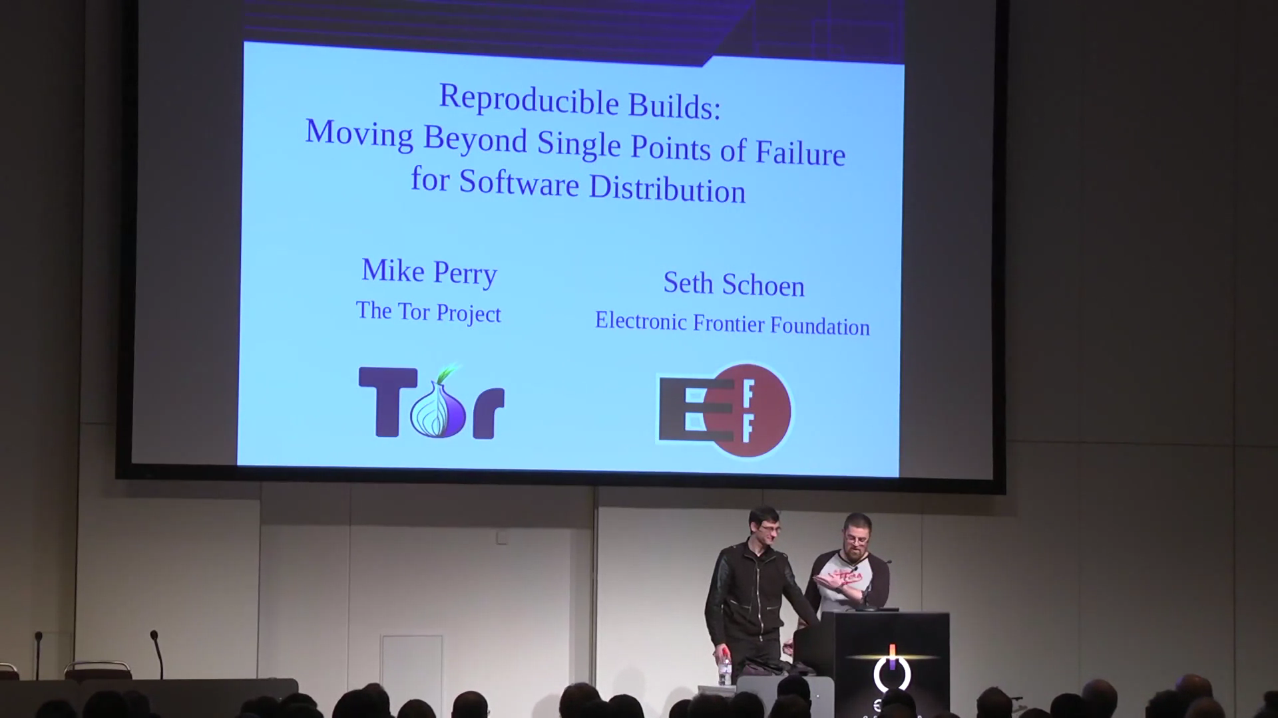
\includegraphics[width=0.7\textwidth]{images/31c3.png}

  Available on \url{media.ccc.de}, 31c3
 \end{center}
\end{frame}

\begin{frame}[fragile]
 \frametitle{Motivations}
 \begin{itemize}
  \item CVE-2002-0083: remote root exploit, 1 bit difference in the binary
  \item 31c3 shows a PoC for a kernel module modifying source code in memory only
  \item how can you be sure what's running on your machine or on a build
  daemon network?
 \end{itemize}
\end{frame}

\begin{frame}[fragile]
 \frametitle{Motivations to crack build machines}
 \begin{itemize}
  \item Compromise one computer to get:
  \begin{itemize}
   \item Hundreds of millions of other computers?
   \item Every bank account in the world?
   \item Every Windows computer in the world?
   \item Every Linux computer in the world?
  \end{itemize}
  \item Compromise one computer is worth:
  \begin{itemize}
   \item \$100k USD (market price of remote 0day)
   \item \$100M USD (censorship budget of Iran per year)
   \item \$4B USD (Bitcoin market cap)
  \end{itemize}
 \end{itemize}
\end{frame}


\begin{frame}[fragile]
 \frametitle{Another example}

 At a CIA conference in 2012:
 \begin{center}
  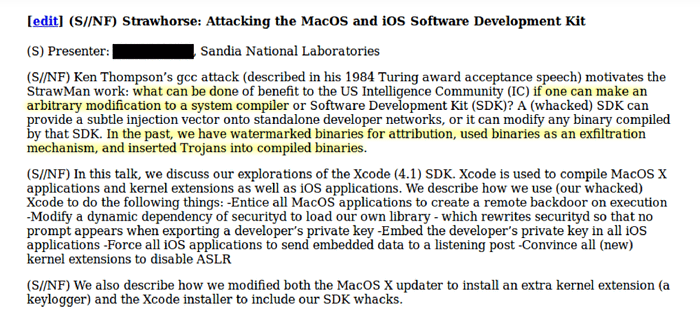
\includegraphics[width=0.8\textwidth]{images/strawhorse.png}

  {\footnotesize
  \url{firstlook.org/theintercept/2015/03/10/ispy-cia-campaign-steal-apples-secrets/}
  }
 \end{center}
\end{frame}

\begin{frame}
 \frametitle{The solution}

 \begin{center}
 \Large
 enable anyone to reproduce\\
 identical binary packages\\
 from a given source
\end{center}

\end{frame}

\begin{frame}
 \frametitle{The solution}

 \begin{center}
 We call this:

 \Huge
 “reproducible builds”
 \end{center}
\end{frame}

\begin{frame}
 \frametitle{It's not only security}

 \begin{itemize}
  \item Early detection of FTBFS and other problems
  \item Debug packages can be created at any time
  \item Smaller \texttt{.deb} deltas
  \item Validation of cross-builds
  \item …
 \end{itemize}
\end{frame}

\begin{frame}
 \frametitle{So trendy!}

 \begin{itemize}
 \item Bitcoin (\textbf{done})
 \item Tor (\textbf{done})
 \item Debian (\emph{in progress})
 \item Coreboot (\textbf{done})
 \item OpenWrt (\emph{in progress})
 \item NetBSD (\emph{in progress})
 \item FreeBSD (\emph{in progress})
 \item Arch Linux (\emph{in progress})
 \item \ldots{}
\end{itemize}

\end{frame}


\begin{frame}[plain]
 \begin{tikzpicture}[remember picture,overlay]
  \node[at=(current page.center)] {
    
\includegraphics[width=\paperwidth]{images/wholeworld.jpg}
    % Credits to Kevin ‘Chuise’ Jackson
    % http://dumhi.com/about
  };
 \end{tikzpicture}
\end{frame}

\begin{frame}[plain]
\begin{center}
 \Huge It should become the \textbf{norm}.\\
 \only<2>{\small We want to change the meaning of "free software": \\
  it's only free software if it is reproducible!}
\end{center}

\end{frame}

\section{Current status}

\begin{frame}[plain]
 \frametitle{Progress in Debian \texttt{unstable}}
 \begin{center}
  \includegraphics[width=\paperwidth]{images/stats_pkg_state.png}
 \end{center}
\end{frame}

\begin{frame}
 \frametitle{What we did since summer 2014}

 \begin{itemize}
  \item Agreed on using a fixed build path: \texttt{/build}
  \item Record the build environment: \texttt{.buildinfo}
  \item \texttt{strip-nondeterminism}
  \item \texttt{reproducible.debian.net}
  \item \texttt{diffoscope} (formerly known as \texttt{debbindiff})
  \item \texttt{SOURCE\_DATE\_EPOCH}
  \item \texttt{disorderfs}
  \item Many many patches: \texttt{dpkg}, \texttt{debhelper}, \texttt{cdbs}, \texttt{sbuild}, …
  \item\only<2>{Tell the world \& collaborate}
 \end{itemize}
\end{frame}


\begin{frame}
 \frametitle{Tell the world \& collaborate}

 \begin{itemize}
  \item Many talks already:
   \begin{itemize}
    \item 2014-02-01: FOSDEM’14
    \item 2014-08-26: DebConf14
    \item 2015-01-31: FOSDEM’15
    \item 2015-07-06: Libre Software Meeting 2015
    \item 2015-08-13: Chaos Communication Camp 2015
    \item 2015-08-20: DebConf15
    \item (videos available, in EN/FR/DE)
   \end{itemize}
  \item More on the wiki:
    {\small \url{https://wiki.debian.org/ReproducibleBuilds/About#Presentations}}
  \item Weekly reports since May 2015
 \end{itemize}
\end{frame}

\begin{frame}
 \frametitle{Tell the world \& collaborate, cont.}

 \begin{itemize}
  \item Summit in December 2015 in Athens
   \begin{itemize}
    \item 40 people from 16 projects
   \end{itemize}
  \item coming soon: \texttt{https://reproducible-builds.org}
  \begin{center}
   
\includegraphics[width=0.6\textwidth]{images/rbwww1.png}
  \end{center}
 \end{itemize}
\end{frame}


\begin{frame}
 \frametitle{Testing for variations}

 \begin{itemize}
  \item Build for the first time
  \item Save the result
  \item Perform change(s) to the environment
  \item Build for a second time
  \item Compare results
  \item\only<2>{started as a 10 line shell script this has become \texttt{reproducible.debian.net}}
 \end{itemize}
\end{frame}

\begin{frame}
 \frametitle{reproducible.debian.net}

 \begin{itemize}
  \item maintained in \texttt{jenkins.debian.net.git}, 27 contributors
  \item 4k lines of Python and 5k lines Bash code
  \item 111 jenkins jobs now running on 10 hosts
  \item Continuously testing Debian testing, unstable and experimental
  \begin{itemize}
   \item Previously amd64 only, now also armhf, more to come…
  \end{itemize}
  \item Not just testing Debian, but also Coreboot, OpenWrt, NetBSD, FreeBSD,
  Archlinux and soon Fedora
  \item Thanks to ProfitBricks for providing amd64 servers:
 \end{itemize}
 \vfill
 \begin{center}
 
\includegraphics[height=0.15\paperheight]{images/profitbricks_logo.png}
 \end{center}
\end{frame}

\begin{frame}[fragile]
 \frametitle{Variations on reproducible.debian.net}

 \begin{center}
  \begin{table}
   \resizebox{0.95\textwidth}{!}{%
    \begin{tabular}{l|ll}
\textbf{variation} & \textbf{first build} & \textbf{second build} \\
\hline
hostname & \texttt{jenkins} & \texttt{i-capture-the-hostname} \\
domainname & \texttt{debian.net} & \texttt{i-capture-the-domainname} \\
\texttt{env TZ} & \texttt{GMT+12} & \texttt{GMT-14} \\
\texttt{env LANG} & \texttt{en\_GB.UTF-8} & \texttt{fr\_CH.UTF-8} \\
\texttt{env LC\_ALL} & not set & \texttt{fr\_CH.UTF-8} \\
\texttt{env USER} & \texttt{pbuilder1} & \texttt{pbuilder2} \\
uid & \texttt{1111} & \texttt{2222} \\
gid & \texttt{1111} & \texttt{2222} \\
UTS namespace & shared with the host & \textit{modified using \texttt{/usr/bin/unshare --uts}} \\
kernel version & Linux 3.16.0-4-amd64 & Linux 2.6.56-4-amd64 \\
umask & 0022 & 0002 \\
CPU type & \multicolumn{2}{l}{same for both builds \textit{(work in progress)}} \\
filesystem & \multicolumn{2}{l}{same for both builds \textit{(work in progress - disorderfs)}} \\
year, month, date & \multicolumn{2}{l}{same for both builds \textit{(work in progress)}} \\
hour, minute & \multicolumn{2}{l}{hour is usually the same… usually, the minute differs… \textit{(work in progress)}} \\
\textit{everything else} & \multicolumn{2}{l}{\textit{is likely the same…}}
    \end{tabular}
   }
  \end{table}
 \end{center}
\end{frame}

\begin{frame}
 \frametitle{reproducible.debian.net}
 \begin{center}
 show in webbrowser
 \end{center}
\end{frame}


\begin{frame}
 \frametitle{Debian .buildinfo}

 \begin{itemize}
  \item Aggregate in the same file:
   \begin{itemize}
    \item Sources (checksums)
    \item Generated binaries (checksums)
    \item Packages used to build (with specific version, checksums coming soon)
   \end{itemize}
  \item Can be later used to reinstall environment exactly as it was
  \item For Debian all versions are available from \url{snapshot.debian.org}
 \end{itemize}
\end{frame}


\begin{frame}[fragile]
 \frametitle{Example .buildinfo}

{\small
\begin{verbatim}
Format: 1.9
Build-Architecture: amd64
Source: txtorcon
Binary: python-txtorcon
Architecture: all
Version: 0.11.0-1
Build-Path: /usr/src/debian/txtorcon-0.11.0-1
Checksums-Sha256:
 a26549d9…7b 125910 python-txtorcon_0.11.0-1_all.deb
 28f6bcbe…69 2039 txtorcon_0.11.0-1.dsc
Build-Environment:
 base-files (= 8),
 base-passwd (= 3.5.37),
 bash (= 4.3-11+b1),
 …
\end{verbatim}
}
\end{frame}


\begin{frame}
 \frametitle{strip-nondeterminism}

 \begin{itemize}
  \item Normalizes various file formats
  \item Currently handles:
   \begin{itemize}
    \item ar archives (\texttt{.a})
    \item gzip
    \item Java jar
    \item Javadoc HTML
    \item Maven \texttt{pom.properties}
    \item PNG
    \item ZIP archives
    \item … \textit{extensible to new formats}
   \end{itemize}
  \item Written in Perl (like \texttt{dpkg-dev})
 \end{itemize}
\end{frame}



{
\usebackgroundtemplate{%
 \begin{tikzpicture}[remember picture,overlay]%
  \node[shift={(-0.15\paperwidth, 0.4\paperheight)},at=(current page.south east)] {
    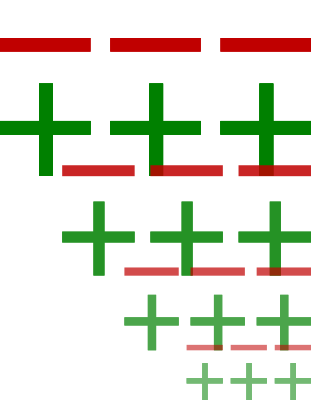
\includegraphics[width=0.2\paperwidth]{images/diffoscope_logo.png}
  };
 \end{tikzpicture}%
}
\begin{frame}{diffoscope}
 \frametitle{Debugging problems: diffoscope}

 \begin{itemize}
  \item Examines differences \textbf{in depth}
  \item Outputs HTML or plain text showing the differences
  \item Recursively unpacks archives
  \item Seeks human readability:
   \begin{itemize}
    \item uncompresses PDF
    \item disassembles binaries
    \item unpacks Gettext files
    \item … \textit{easy to extend to new file formats}
   \end{itemize}
  \item Falls back to binary comparison
  \item Available in Debian sid and stretch
  \item Maintainers in other distros wanted
 \end{itemize}
 \vfill
 \begin{center}
  \url{http://diffoscope.org/}\\
  {\footnotesize \color{gray}{(formely known as \texttt{debbindiff})}}
 \end{center}
\end{frame}
}

\begin{frame}
 \frametitle{diffoscope example (HTML output)}

 \begin{center}
  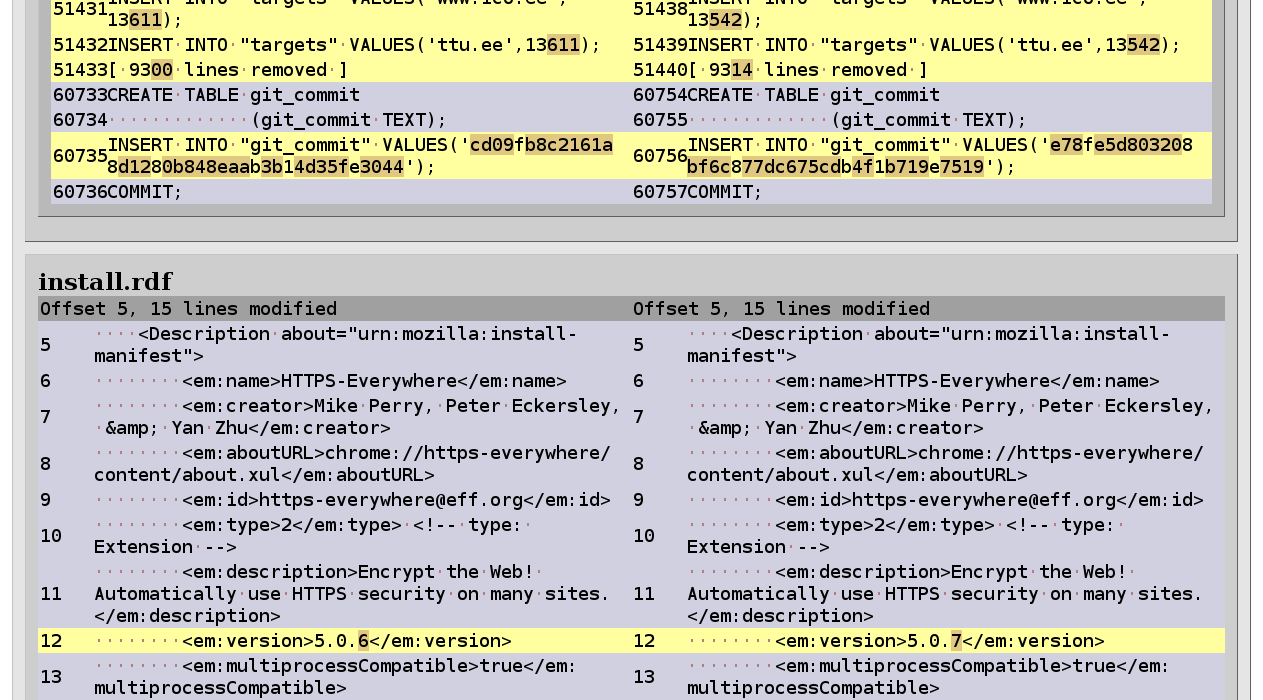
\includegraphics[width=0.9\paperwidth]{images/diffoscope_example_html.png}
 \end{center}
\end{frame}

\begin{frame}
 \frametitle{diffoscope example (text output)}

 \begin{center}
  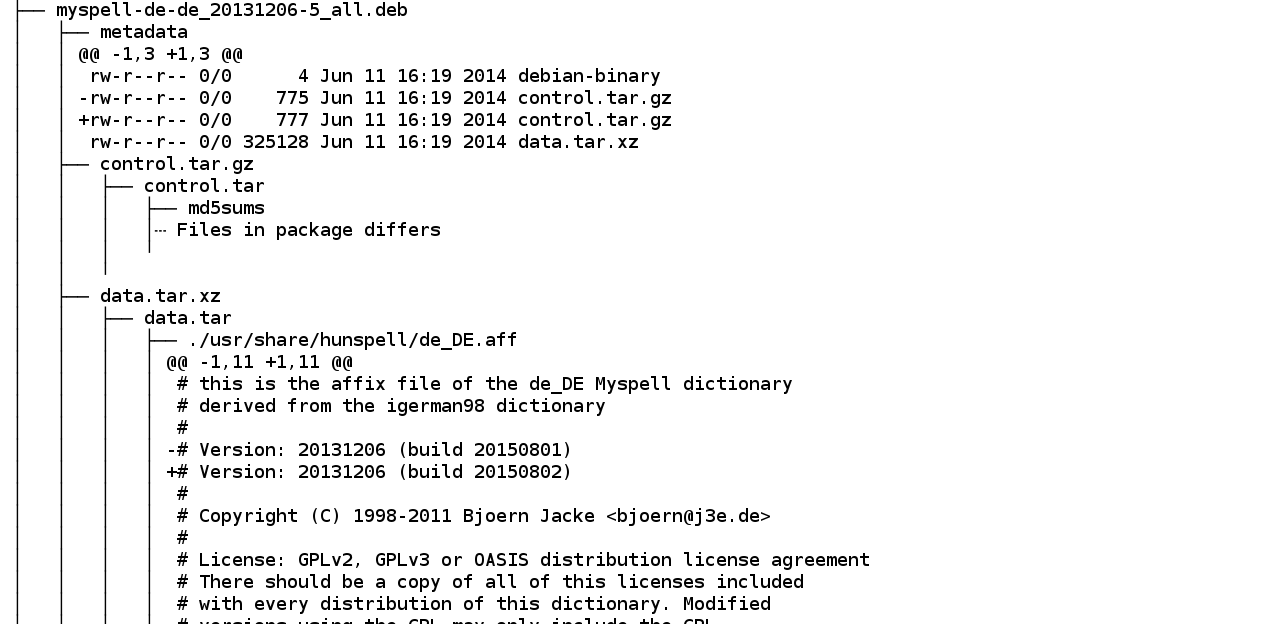
\includegraphics[width=0.9\paperwidth]{images/diffoscope_example_text.png}
 \end{center}
\end{frame}

\begin{frame}
 \frametitle{\texttt{SOURCE\_DATE\_EPOCH}}

 \begin{itemize}
  \item Build date usually not useful for the user
  \item Standardize a build-time environment variable
  \item Value of \texttt{SOURCE\_DATE\_EPOCH} is used instead of the current date
  \item General solution for other free software projects and distributions
  \item In Debian, set from the latest \texttt{debian/changelog} entry
 \end{itemize}
\end{frame}

\begin{frame}
 \frametitle{\texttt{SOURCE\_DATE\_EPOCH} (closed bugs)}

 \begin{itemize}
  \item \texttt{\#787444}: help2man
  \item \texttt{\#790899}: epydoc
  \item \texttt{\#794004}: ghostscript
  \item \texttt{\#783475}: texi2html
  \item sphinx \small{\url{https://github.com/sphinx-doc/sphinx/pull/1954}}
 \end{itemize}

\end{frame}

\begin{frame}
 \frametitle{\texttt{SOURCE\_DATE\_EPOCH} (open bugs)}

 \begin{itemize}
  \item \texttt{\#792201}: doxygen
  \item \texttt{\#790801}: txt2man
  \item \texttt{\#791815}: libxslt
  \item \texttt{\#792687}: gettext (xgettext)
  \item \texttt{\#794681}: qt4-x11 (qthelpgenerator)
  \item \texttt{\#794586}: ocamldoc
  \item \texttt{\#792202}: texlive-bin
  \item gcc (\texttt{\_\_DATE\_\_} and \texttt{\_\_TIME\_\_} macros) \texttt{\footnotesize{\url{https://gcc.gnu.org/ml/gcc-patches/2015-06/msg02210.html}}}
 \end{itemize}

\end{frame}

\section{Fixing reproducibility issues}

% Straightforward..

\begin{frame}{Timestamps in gzip headers}
 \begin{center}
  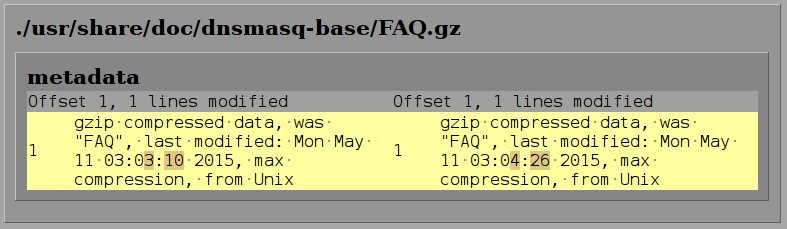
\includegraphics[width=0.9\textwidth]{images/examples/timestamps_in_gzip.png}
  \vfill
  \pause
  \texttt{gzip FAQ} $\Longrightarrow$ \texttt{gzip -n FAQ}
 \end{center}
\end{frame}

\begin{frame}{Timestamps in Python version}
 \begin{center}
  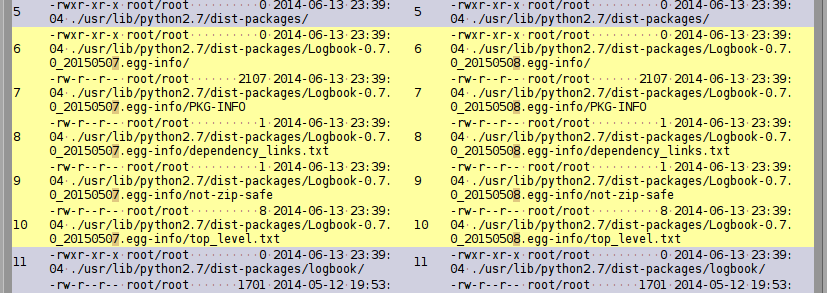
\includegraphics[width=0.9\textwidth]{images/examples/timestamps_in_python_version.png}
  \vfill
  \texttt{tag\_date=True} $\Longrightarrow$ \texttt{tag\_date=False} in \texttt{setup.py}
 \end{center}
\end{frame}

\begin{frame}{Timestamps in static libraries}
 \begin{center}
  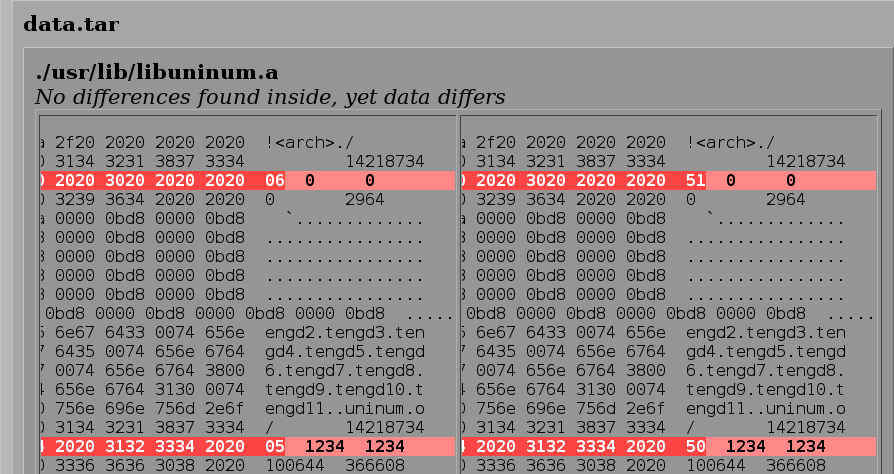
\includegraphics[width=0.7\textwidth]{images/examples/timestamps_in_static_library.png}
  \vfill
  \texttt{.a} files are "\texttt{ar}" archives $\Longrightarrow$ \texttt{binutils} in determinstic mode or \texttt{strip-nondeterminism}
 \end{center}
\end{frame}

\begin{frame}{Timestamps in PNG}
 \begin{center}
  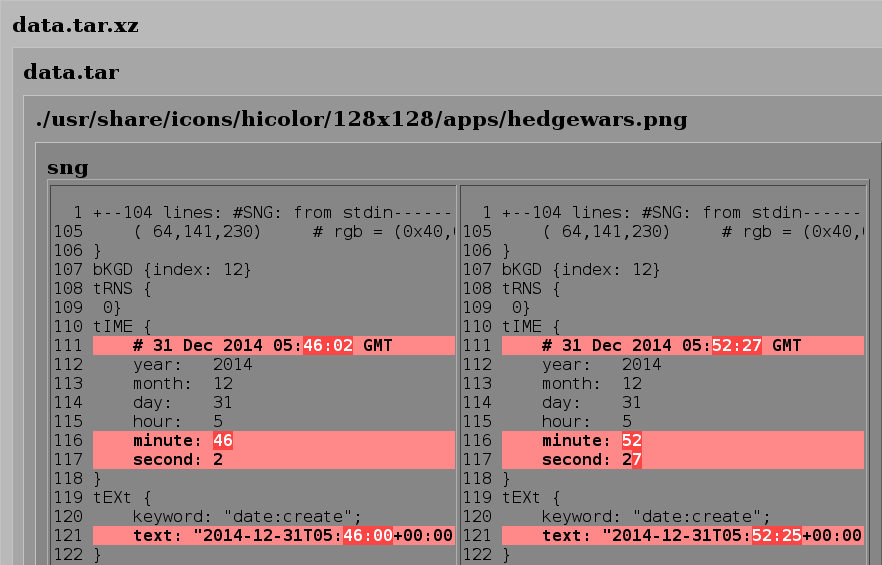
\includegraphics[width=0.6\textwidth]{images/examples/timestamps_in_png.png}
  \vfill
  \texttt{convert ... +set date:create +set date:modify -define png:exclude-chunk=time}
 \end{center}
\end{frame}

\begin{frame}{Tarballs: Users and groups}
 \begin{center}
  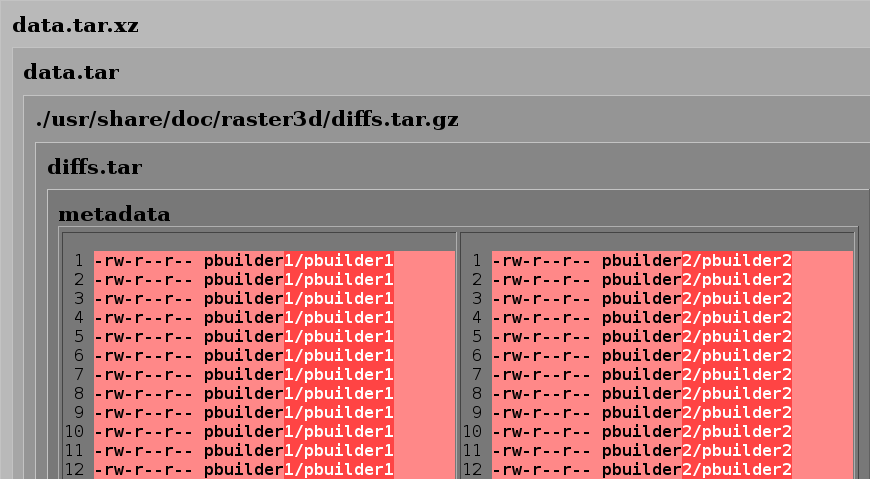
\includegraphics[width=0.7\textwidth]{images/examples/user_and_group_in_tarball.png}
  \vfill
  \texttt{--owner=root --group=root --numeric-owner}
 \end{center}
\end{frame}

\begin{frame}{Tarballs: Ordering}
 \begin{center}
  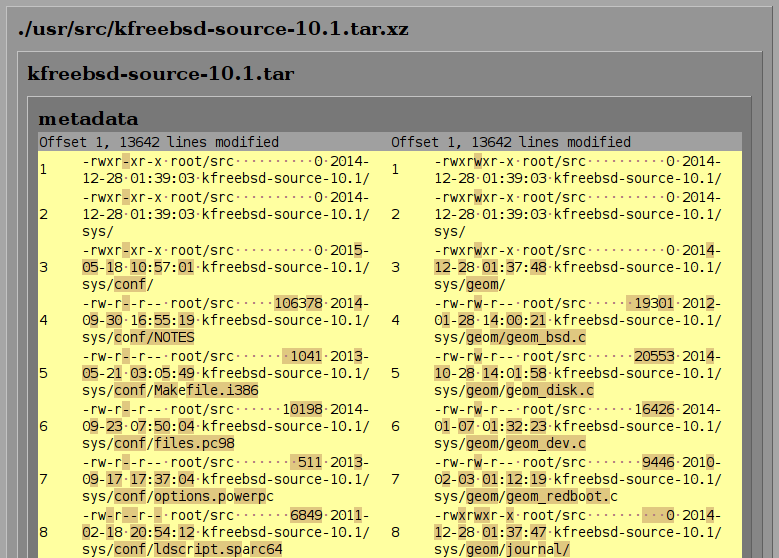
\includegraphics[width=0.6\textwidth]{images/examples/random_order_in_tarball.png}
  \vfill
  \texttt{find -type f | LC\_ALL=C sort | tar ...}
 \end{center}
\end{frame}

\begin{frame}{Tarballs: Timestamps}
 \begin{center}
  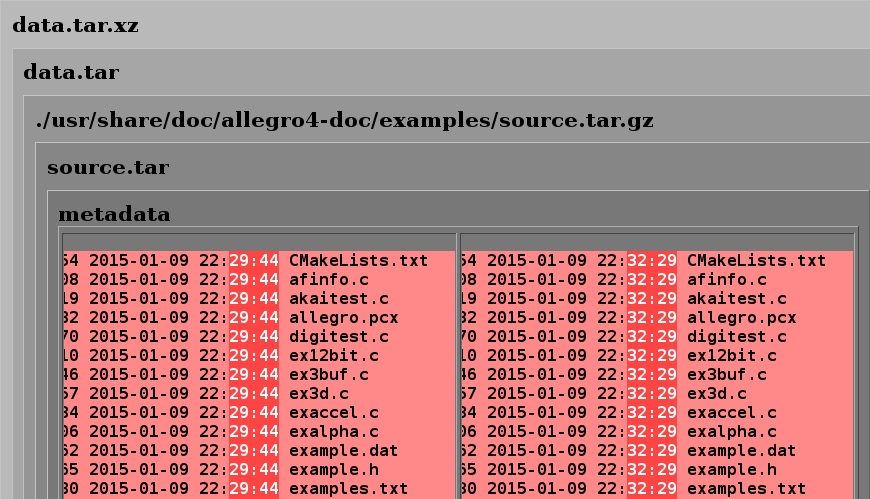
\includegraphics[width=0.7\textwidth]{images/examples/timestamps_in_tarball.png}
  \vfill
  $\Longrightarrow$ \texttt{--mtime} (or \texttt{find}/\texttt{xargs}/\texttt{touch})
 \end{center}
\end{frame}

% toolchain

\begin{frame}{Timestamps in Erlang .BEAM}
 \begin{center}
  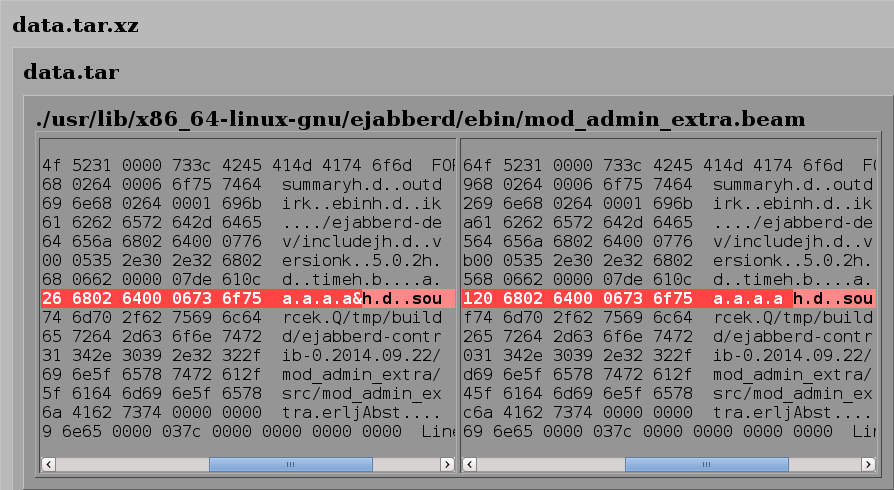
\includegraphics[width=0.6\textwidth]{images/examples/timestamps_in_beam.png}
  \vfill
  \vfill
  Patch \texttt{erlc} to obey \texttt{SOURCE\_DATE\_EPOCH} (\texttt{\#795834})
 \end{center}
\end{frame}

\begin{frame}{Timestamps in Ruby gemspec}
 \begin{center}
  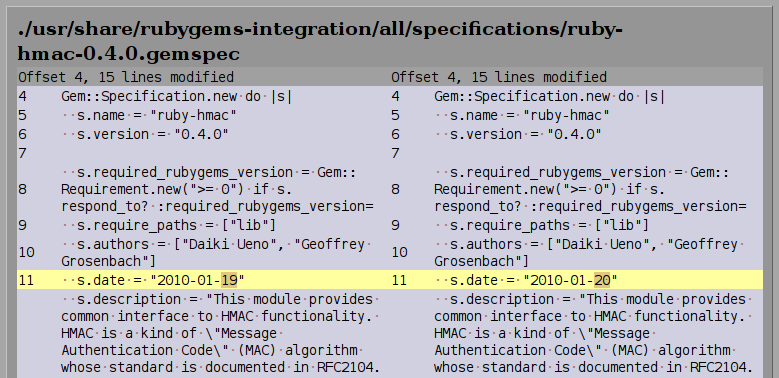
\includegraphics[width=0.9\textwidth]{images/examples/timestamps_in_ruby_gemspec.png}
  \vfill
  Varies on timezone $\Longrightarrow$ patch to always use UTC (\texttt{\#779631})
 \end{center}
\end{frame}

% ugly

\begin{frame}{Hostname/time recorded via ./configure}
 \begin{center}
  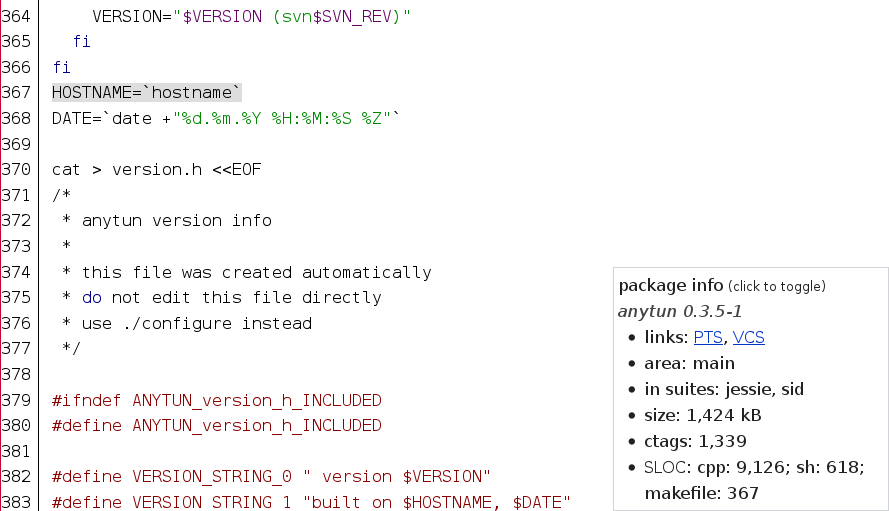
\includegraphics[width=0.7\textwidth]{images/examples/hostname_in_configure.png}
  \vfill
  $\Longrightarrow$ Sometimes override from \texttt{debian/rules}..?
 \end{center}
\end{frame}

% uglier

\begin{frame}{Perl hash order}
 \begin{center}
  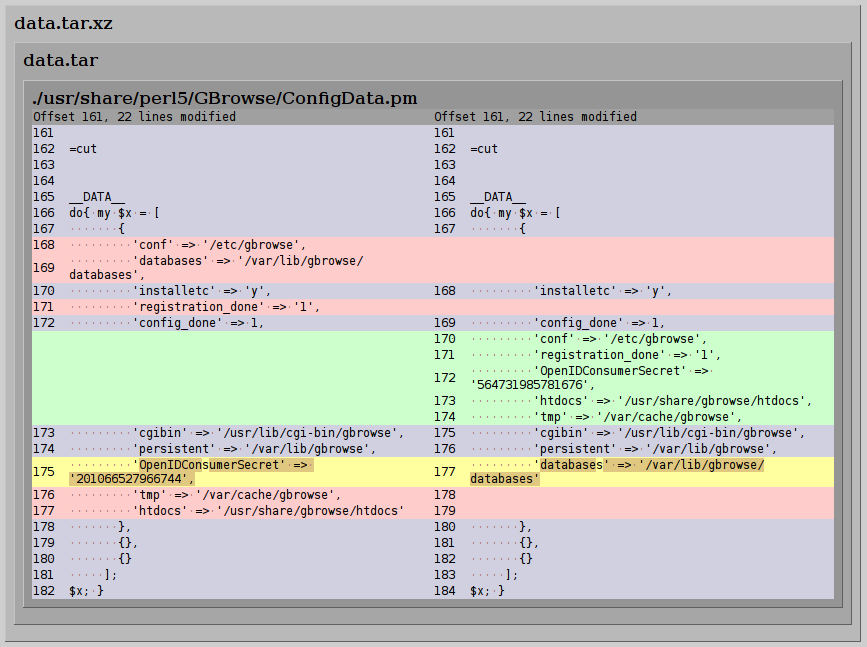
\includegraphics[width=0.6\textwidth]{images/examples/random_perl_hash_order.png}
  \vfill
  $\Longrightarrow$ \texttt{\$Data::Dumper::Sortkeys = 1;}
 \end{center}
\end{frame}

\begin{frame}{Timestamps in header files}
 \begin{center}
  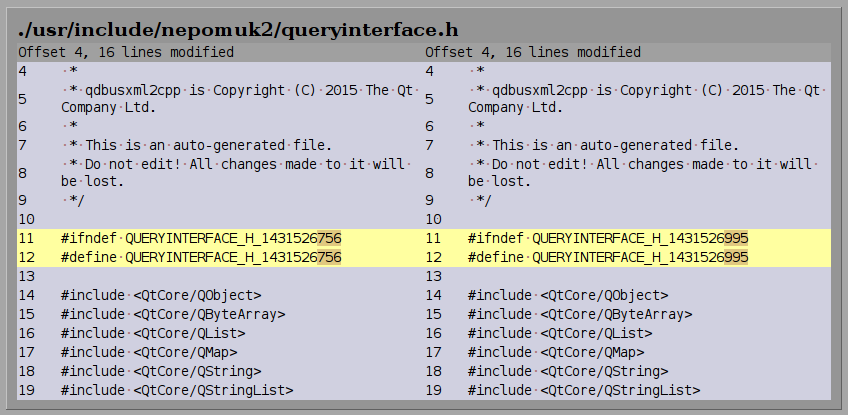
\includegraphics[width=0.6\textwidth]{images/examples/timestamps_in_header_files.png}
  \vfill
  Patch with a better unique id or use \texttt{SOURCE\_DATE\_EPOCH}
 \end{center}
\end{frame}

\begin{frame}{Build time recorded via Makefile}
 \begin{center}
  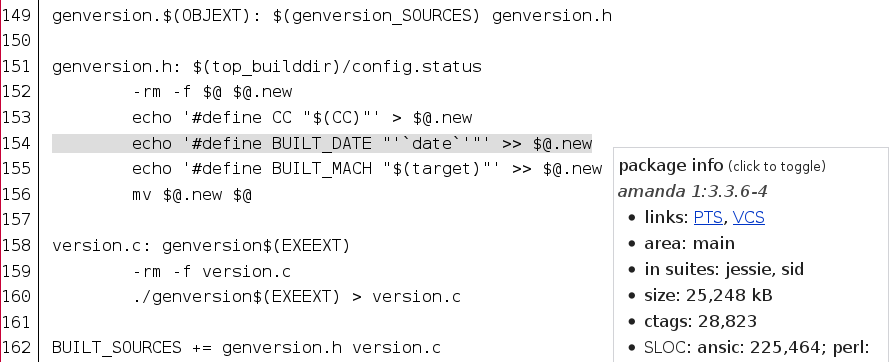
\includegraphics[width=0.9\textwidth]{images/examples/build_date_in_makefile.png}
  \vfill
  $\Longrightarrow$ Patch upstream\ldots{} :(
 \end{center}
\end{frame}

\begin{frame}
 \frametitle{Some toolchain issues}

 % list taken from https://wiki.debian.org/ReproducibleBuilds/ExperimentalToolchain on 2015-08-19
 % Skipping SOURCE_DATE_EPOCH related patches since they are listed in the related section
 \begin{itemize}\small
  \item \sout{\texttt{\#776026} \textbf{wheel:} create reproducible wheel (.whl) files}
  \item \sout{\texttt{\#776143} \textbf{docbook-to-man:} remove timestamps from the generated manpages}
  \item \sout{\textbf{gtk-doc:} generate its links in a stable order}
  \item \texttt{\#774148} \textbf{fontforge:} propagate creation and modification times from source file
  \item \texttt{\#775786} \textbf{python-support:} sort file lists in /usr/share/python-support/*.private
  \item \textbf{libxslt:} make generate-id() return identifiers in a deterministic way
  \item And many more! \url{https://deb.li/3bX6F}
 \end{itemize}
\end{frame}

\begin{frame}
 \frametitle{Work on individual packages}

 \begin{itemize}
  \item 644 bugs for individual problems
  \item 610 tagged with “patch”
  \item Nearly two patches per day since fall 2014 on average!
 \end{itemize}
\end{frame}

\begin{frame}[plain]
 \begin{tikzpicture}[remember picture,overlay]
  \node[at=(current page.center)] {
    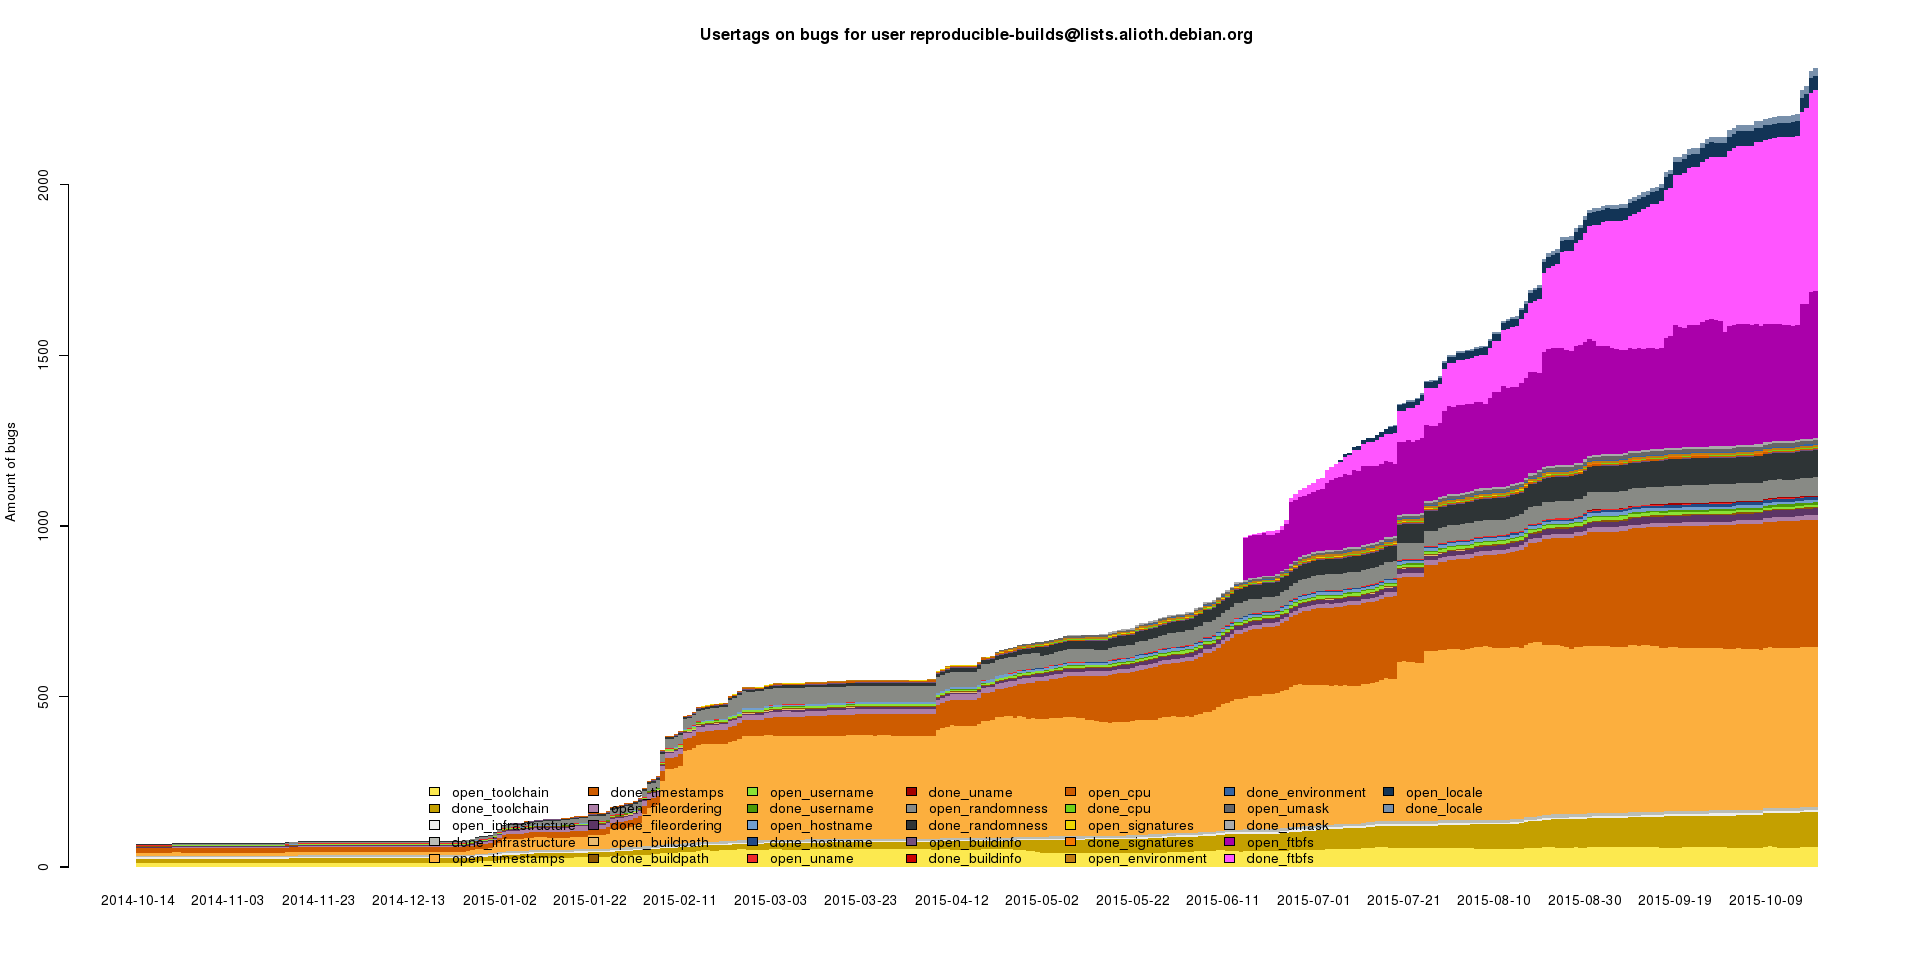
\includegraphics[width=\paperwidth]{images/stats_bugs.png}
  };
 \end{tikzpicture}
\end{frame}

\section{Next?}

\begin{frame}
 \frametitle{Status and next steps in Debian}
 \begin{itemize}
  \item Remember: this is just a proof-of-concept, Debian is not 80\%
  reproducible.
  \item Major changes still need to be merged.
  \item Once this has happend, Debian will be >80\% reproducible.
  \item The next Debian release ("stretch") shall be >80\% reproducible.
 \end{itemize}
\end{frame}

\begin{frame}
 \frametitle{dpkg}

 \begin{itemize}\small
  \item \sout{\texttt{\#719844}: make compression of \{data,control\}.tar.gz deterministic}
  \item \texttt{\#759999}: set reproducible timestamps in \texttt{.deb} ar file headers
  \item \texttt{\#787980}: normalize file permissions when creating control.tar
  \item \texttt{\#719845}: make file order within {data,control}.tar.gz deterministic
  \item \texttt{dpkg-genbuldinfo}: \textit{patch already written, but waiting on agreement about spec}
 \end{itemize}
\end{frame}

\begin{frame}
 \frametitle{debhelper}

 \begin{itemize}\small
  \item \texttt{\#759886}: make mtimes of packaged files deterministic
  \item \texttt{\#759895}: add a call to \texttt{dh\_strip\_nondeterminism} in \texttt{dh}
  \item \texttt{\#791823}: set \texttt{SOURCE\_DATE\_EPOCH} env var for reproducible builds
 \end{itemize}
\end{frame}

\begin{frame}
 \frametitle{cdbs}

 \begin{itemize}\small
  \item \texttt{\#794241}: export \texttt{\$SOURCE\_DATE\_EPOCH} to produce reproducible output
 \end{itemize}
\end{frame}

\begin{frame}
 \frametitle{sbuild}

 \begin{itemize}\small
  \item \texttt{\#790868}: allow sbuild to use a deterministic build path to build packages
  \item \texttt{\#778571}: predictible build location for reproducible builds
  \item Finish the \texttt{srebuild} script
 \end{itemize}
\end{frame}

\begin{frame}
 \frametitle{ftp.debian.org}

 \begin{itemize}\small
  \item \texttt{\#763822}: please include .buildinfo file in the archive
 \end{itemize}
\end{frame}

\begin{frame}
 \frametitle{"Finally", changing Debian policy}

 \begin{itemize}
  \item Section 4.15: “Sources must build in a reproducible binaries.” 
 \end{itemize}
\end{frame}


\begin{frame}
 \frametitle{Next steps in other distributions}
 \begin{itemize}
  \item Yo que se
  \item seriously: I don't know. 
  \item 2016 will be a very interesting year.
 \end{itemize}
\end{frame}

\begin{frame}
 \frametitle{Reproducible builds are just the beginning}
 \begin{itemize}
  \item Re-creating the build environment is mandatory too, and only really solved
  for Debian so far.
 \end{itemize}
\end{frame}

\begin{frame}
 \frametitle{Reproducible builds are just the beginning, cont.}
 \begin{itemize}
  \item Continuous rebuilds need to happen in a systematic way and the
  results need to be properly published.
  \item\only<2>{ Integration in end user tools\\
  "Do you really want to install this unreproducible software (y/N)" \\
  "Which rebuilders do you want to trust?"}
 \end{itemize}
\end{frame}


\section{Want to help?}

\begin{frame}
 \frametitle{As a software developer}
 \begin{itemize}
  \item stop using build date
  \item use \texttt{SOURCE\_DATE\_EPOCH} instead \\
  \item see  \url{https://reproducible-builds.org/specs/}
 \end{itemize}
\end{frame}

\begin{frame}
 \frametitle{Get involved - learning by doing}

 \begin{itemize}
  \item Test for yourself:
   \begin{itemize}
    \item just build something twice, run diffoscope on the results
    \begin{itemize}
     \item for better results use our “reproducible” repository, \texttt{pbuilder} and a custom config
    \end{itemize}
   \end{itemize}

  \item Tips on the wiki: \\
    {\small \url{https://wiki.debian.org/ReproducibleBuilds/Howto}} \\
    {\small
    \url{https://wiki.debian.org/ReproducibleBuilds/ExperimentalToolchain}}
  \item Ask for help on \texttt{\#debian-reproducible} \\
   or on the mailing-list
 \end{itemize}
\end{frame}

\begin{frame}
 \frametitle{Join the team!}

 \begin{itemize}
  \item Why?
   \begin{itemize}
    \item \heartsuit{}\heartsuit{}\heartsuit{} Lovely group of people \heartsuit{}\heartsuit{}\heartsuit{}
    \item Learn something new everyday
    \item Change the (software) world!
   \end{itemize}
  \item What do we do?
   \begin{itemize}
    \item Review packages
    \item Identify issues and document solutions
    \item \texttt{reproducible.d.n}, diffoscope, strip-nondeterminism
    \item Propose changes for toolchain
    \item Submit patches for individual packages
    \item Write more general documentation and  talk to the world
   \end{itemize}
 \end{itemize}
\end{frame}

\begin{frame}
 \frametitle{Create a new team!}

 \begin{itemize}
  \item Why?
   \begin{itemize}
    \item Every distribution should be reproducible!
    \item Learn something new everyday
    \item Change the (software) world!
   \end{itemize}
  \item How to get started?
   \begin{itemize}
    \item Talk to me here or talk to us on IRC or via mail.
    \item RTFM, there is lots of documentation
    \item Experiment - learning by doing
   \end{itemize}
 \end{itemize}
\end{frame}

\begin{frame}
 \frametitle{Write a thesis!}

 \begin{itemize}
  \item We are trying to document all our work, but we won't write
  scientific articles.
  \item Maybe you can do that?
  \item We'll be happy to help and there is Gunnar Wolf (gwolf@debian.org) in
  Mexico, D.F. too!
 \end{itemize}
\end{frame}


\section{Questions?}

\begin{frame}
 \frametitle{Questions?}
 \begin{center}
  Please ask me now or later today.
 \end{center}
 \begin{itemize}
 \item\url{https://reproducible.debian.net}
 \item\url{#debian-reproducible} on \url{irc.OFTC.net}
 \end{itemize}
\end{frame}

\begin{frame}
 \frametitle{Thanks!}

 \begin{itemize}
  \item Debian “Reproducible Builds” team \\
        {\small (you are just \textbf{so} awesome!)}
  \item Linux Foundation and the Core Infrastructure Initiative
  \item Congreso de seguridad de la información
\end{itemize}

 \begin{center}
  
\includegraphics[height=0.1\paperheight]{images/linux_foundation_logo.png}
  \hspace{0.1\paperwidth}
  
\includegraphics[height=0.1\paperheight]{images/cii_logo.png}
 \end{center}

 \vfill
 \begin{center}
  \resizebox{0.8\textwidth}{!}{%
   \begin{tabular}{rl}
    \texttt{holger@debian.org} & \texttt{B8BF 5413 7B09 D35C F026} \\
                               & \texttt{FE9D 091A B856 069A AA1C}
   \end{tabular}
  }
 \end{center}
\end{frame}

\end{document}
